\documentclass[11pt]{article}  % article/book/letter/report/...

\usepackage{geometry}
\geometry{
    top=30mm,
    left=30mm,
    right=30mm
}

\usepackage{palatino}
\usepackage{amsmath}
\usepackage{bm}
\usepackage{amssymb}
\usepackage{mathtools}
\usepackage{commath}
\usepackage{mathpazo}
\usepackage{graphicx}
\usepackage{subcaption}
\usepackage{float}
\usepackage{textcomp}
\usepackage{siunitx}
\usepackage{setspace}
\usepackage{hyperref}
\usepackage{listings}
\usepackage{color}
\usepackage{enumitem}
\usepackage{gensymb}

\definecolor{darkgreen}{rgb}{0,0.6,0}
\definecolor{gray}{rgb}{0.5,0.5,0.5}
\definecolor{mauve}{rgb}{0.58,0,0.82}

\lstset{
    language=python,                          % the language of the code
    numbers=left,                             % where to put the line-numbers
    numberstyle=\tiny\color{gray},            % style of the line-numbers. \footnotesize\color{darkgray} is smaller
    stepnumber=1,                             % the step between two line-numbers. if set to 1, each line will be numbered
    numbersep=5pt,                            % how far the line-numbers are from the code
    backgroundcolor=\color[RGB]{247,255,251}, % background color. \color[RGB]{245,245,244} is a little bit darker than white
    showspaces=false,                         % if set to true, underscores will be shown to indicate spaces
    showstringspaces=false,                   % if set to true, underscores will be shown to indicate spaces within strings
    showtabs=false,                           % if set to true, underscores will be shown to indicate tabs within strings
    frame=single,                             % add a frame around the code, if set to none, no frame will be displayed
    rulecolor=\color{black},                  % frame-color
    tabsize=4,                                % set default tabsize to 4 spaces
    captionpos=b,                             % set the caption-position to bottom
    breaklines=true,                          % set automatic line breaking
    breakatwhitespace=false,                  % set if automatic breaks should only happen at whitespace
    title=\lstname,                           % show the filename of the script included with \lstinputlisting
    keywordstyle=\color{blue},                % keyword style. \color[RGB]{40,40,255} is dark blue
    escapeinside={\%*}{*)},                   % if you want to add LaTeX within your code
    morekeywords={*,...},                     % if you want to add more keywords to the set
    basicstyle=\ttfamily\scriptsize,          % source code style
    commentstyle=\ttfamily\color{darkgreen},  % comment style. \it\color[RGB]{0,96,96} is italic dark green
    stringstyle=\ttfamily\color{mauve}        % string literal style. also try \rmfamily\slshape\color[RGB]{128,0,0}
}

\usepackage[type={CC}, modifier={by-nc-sa}, version={3.0},]{doclicense}

\title{3D Math Review Practice}
\author{\href{mailto:neo-mashiro@hotmail.com}{\color{purple}{Wentao Lu}}}
\date{2020-09-15}

\begin{document}
    \newcommand{\solution}{\noindent \textbf{\textsc{Solution:}} \dotfill \vspace{2mm}}  % solution title
    \definecolor{purple}{rgb}{0.4,0,0.8}

    \maketitle
    \pagenumbering{arabic}

\section{Pinhole Camera Model}
    For a pinhole camera, the focal length is the distance from the pinhole to the film plane. The dimensions of a frame of 35-mm film are about 24mm$\times$36mm (width$\times$height). The field of view of the pinhole camera is the angle made by the largest object that the camera can image on its film plane, but a real field of view is hard to deal with, so people use surface angles of view such as the one in the xz-plane, the yz-plane, or in the planes passing through one of the diagonals of the film plane. Assume that the human visual system has an angle of view of 90\textdegree, what focal length should we use with 35-mm film to achieve a natural view in
    \begin{enumerate}[itemsep=0mm]
        \item the xz-plane?
        \item the yz-plane?
        \item any of the planes passing through one of the diagonals of the film plane?
    \end{enumerate}
    For any 3D point $(x,y,z)$ lying in the field of view of the pinhole camera with focal length $d$, what is the projected point $(u,v)$ onto the film plane?\vspace{3mm}

\solution\\
    A sectional view of the pinhole camera model consists of two pairs of similar right triangles. To achieve a natural view when the human visual system has 90\textdegree\hspace{0pt} field of view, the surface angle of view in any plane must also be 90\textdegree, so the interior angles of these triangles are 90/2 = 45\textdegree. Since $tan45$ is 1, the height and base of the triangle must be equal, so in our case, the focal length $d$ = $h/2$, where $h$ is the height of the triangle.\\

    \noindent For the xz-plane, $h$ is the width of the 35-mm film frame along x-direction, which is 24mm, so $d = 12$mm. For the yz-plane, $h$ is the height along y-direction, which is 36mm, so $d = 18$mm. For the plane that passes through the diagonals, the diagonal length will substitute for $h$, so $d$ is half of $\sqrt{24^2+36^2}$ which is 21.63mm.\\

    \noindent For perspective projection, the result coordinates onto the image plane are
    \begin{align*}
        u = -\frac{xd}{z},\; v = -\frac{yd}{z}
    \end{align*}

\section{Lookup Table}
    If we use direct coding of \textsc{rgb} values with 10 bits per primary color, how many possible colors do we have for each pixel? If we use 12-bit pixel values in a lookup table representation, how many entries does the lookup table have?\vspace{3mm}

\solution\\
    10 bits in each \textsc{Rgb} channel allows $2^{10}$ = 1024 colors, so we have $2^{30}$ possible colors for each pixel. 12-bit pixel values can store $2^{12}$ = 4096 indices of the lookup table, so the table has 4096 entries, each encodes a true \textsc{Rgb} color.

\section{Vectors and Planes}
    \begin{enumerate}[leftmargin=*]
        \item Find the equation of the plane determined by the three points:\vspace{3mm}\\
        $\diamond\; P_0(1, 5,-7)\;$
        $\diamond\; P_1(2, 6, 1)\;$
        $\diamond\; P_2(0, 1, 2)\;$
        \item Find the equation of the line passing through $P_0(1,-5,2)$ and $P_1(6,7,-3)$.
        \item Let a plane be determined by the normal $n(1,-1,1)$ and the point $P_0(2,3,-1)$. Find the distance from point $P(5,2,7)$ to the plane.
        \item Given the plane $5x - 3y + 6z - 7$ = 0, find a normal vector to the plane, determine whether $P_1(1,5,2)$ and $P_2(-3,-1,2)$ are on the same side of the plane.
    \end{enumerate}

\solution
    \begin{enumerate}[leftmargin=*, topsep=0pt]
        \item We can find a normal of the plane using the cross product of two vectors:
        \begin{align*}
            n = \overrightarrow{P_0P_1} \times \overrightarrow{P_1P_2} = (1,1,8)\times(-2,-5,1) = (41,-17,-3)
        \end{align*}
        so the plane equation can be written as:
        \begin{align*}
            41x - 17y - 3z + D = 0
        \end{align*}
        plug $P_2(0,1,2)$ into the equation and solve for $D$, we have $D=23$, so the equation is:
        \begin{align*}
            41x - 17y - 3z + 23 = 0
        \end{align*}
        
        \item $\overrightarrow{P_0P_1}$ = $(5,12,-5)$, so the equation of the line can be written as:
        \begin{align*}
            \frac{x-x_1}{5} = \frac{y-y_1}{12} = \frac{z-z_1}{-5}
        \end{align*}
        substitute in $P_0(1,-5,2)$, so we have
        \begin{align*}
            \frac{x-1}{5} = \frac{y+5}{12} = \frac{z-2}{-5}
        \end{align*}

        \item The distance from $P(5,2,7)$ to the plane is the projected length of $\overrightarrow{P_0P}$ onto the normal
        \begin{align*}
            \frac{|\overrightarrow{P_0P} \cdot n|}{|n|} = \frac{|(3,-1,8) \cdot (1,-1,1)|}{\sqrt{1^2+(-1)^2+1^2}} = \frac{12}{\sqrt{3}} = 4\sqrt{3}
        \end{align*}

        \item One of the normal vector is simply $n$ = $(5,-3,6)$. Randomly choose a point on the plane, such as $P_0(-1,0,2)$, we have two vectors from $P_0$
        \begin{align*}
            \overrightarrow{P_0P_1} = (2,5,0),\;\; \overrightarrow{P_0P_2} = (-2,-1,0)
        \end{align*}
        whose dot products with the normal vector are
        \begin{align*}
            \overrightarrow{P_0P_1} \cdot n &= (2,5,0)\cdot(5,-3,6) = -5 < 0\\
            \overrightarrow{P_0P_2} \cdot n &= (-2,-1,0)\cdot(5,-3,6) = -7 < 0
        \end{align*}
        Since both of them yield a negative dot product, it implies that they are in the opposite direction from the normal, and their angles from the normal are between 90\textdegree\hspace{0mm} and 180\textdegree. Hence, $P_1$ and $P_2$ must be on the same side of the plane. (if the dot product is 0, the point lies on the plane)
    \end{enumerate}

\section{Collinearity and Convexity}
    \begin{enumerate}[leftmargin=*]
        \item Three vertices (in 3D) determine a triangle if they do not lie in the same line. Devise a test for collinearity of three vertices.
        \item Given a set of vertices, find a test to determine whether the polygon that they determine is planar or not.
        \item Devise a test for the convexity of a two-dimensional polygon.
    \end{enumerate}

\solution
    \begin{enumerate}[leftmargin=*, topsep=0pt]
        \item Consider three arbitrary vertices $P_1(x_1,y_1,z_1)$, $P_2(x_2,y_2,z_2)$, $P_3(x_3,y_3,z_3)$. If they are collinear, one vertex is the linear combination of the other two, so
        \begin{align*}
            \det{\begin{bmatrix}
                x_1 & x_2 & x_3\\
                y_1 & y_2 & y_3\\
                z_1 & z_2 & z_3
            \end{bmatrix}} = 0
        \end{align*}
        
        \item Pick three vertices at random, if they are not collinear, they uniquely determine a plane. Next, evaluate the plane equation for all other vertices, if it evaluates to 0, the vertex must be on the same plane, otherwise the polygon is not planar.
        
        \item This is similar to what we did to find the convex hull. Given a two-dimensional polygon, we start from a random vertex and traverse along the sides of the polygon in a clockwise manner, for each side we visit, define the side as a vector in the forward direction. If the polygon is convex, we must be making only right turns in each step.

        Mathematically, we can check this by computing the dot product of adjacent vectors as we traverse. Consider two adjacent vectors $v_1$ and $v_2$, and $v_2'$ is the vector of $v_2$ rotated by 90\textdegree\hspace{0mm} clockwise, then $v_2$ is on the right hand side of $v_1$ if and only if
        \begin{enumerate}[itemsep=0mm]
            \item[(1)] $v_1 \cdot v_2 \geq 0$
            \item[(2)] $v_1 \cdot v_2' \leq 0$
        \end{enumerate}
    \end{enumerate}

\section{Transformations}
    %%%%%%%%%%%%%%%%%%%%%%%%%%%%%%%%%%%%%%%%%%%%%%%%%%%%%%%%%%%%%%%%%%%%%%%%%%%%%%%%%%%%%%%%%%%%%%%
    \begin{enumerate}[leftmargin=*]
        \item[\textcolor{blue}{1.}] Prove that a y-reflection (reflection about the x-axis) followed by a reflection through the line $y$ = $-x$ is a pure rotation.
    \end{enumerate}
    
    \solution
    
    The reflection matrix about the x-axis is $r_1 = $
    $\begin{psmallmatrix}
        1 & 0\\0 & -1
    \end{psmallmatrix}$
    
    The reflection matrix about line $y = -x$ is $r_2 = $
    $\begin{psmallmatrix}
        0 & -1\\-1 & 0
    \end{psmallmatrix}$\\
    
    $r_1 \cdot r_2 = $
    $\begin{pmatrix}
        1 & 0\\0 & -1
    \end{pmatrix}$
    $\begin{pmatrix}
        0 & -1\\-1 & 0
    \end{pmatrix}$
    $=$
    $\begin{pmatrix}
        0 & -1\\1 & 0
    \end{pmatrix}$
    is a rotation around the z-axis by 90\textdegree\hspace{0mm}.\\
    
    %%%%%%%%%%%%%%%%%%%%%%%%%%%%%%%%%%%%%%%%%%%%%%%%%%%%%%%%%%%%%%%%%%%%%%%%%%%%%%%%%%%%%%%%%%%%%%%
    \begin{enumerate}[leftmargin=*]
        \item[\textcolor{blue}{2.}] Find the vertices of the rotated triangle obtained by performing a 45\textdegree\hspace{0mm} rotation of triangle $A(0,0)$, $B(1,1)$, $C(5,2)$.
        \begin{enumerate}[leftmargin=6.5mm]
            \item about the origin
            \item about $P(-1,-1)$
        \end{enumerate}
    \end{enumerate}
    
    \solution
    
    Let $s=sin45$, $c=cos45$, $\Rightarrow$ a 45\textdegree\hspace{0mm} counter-clockwise rotation is given by
    \begin{align*}
        \begin{pmatrix}
            c & s\\-s & c
        \end{pmatrix}
        \;\;\text{where}\; s = c = \frac{\sqrt{2}}{2}
    \end{align*}
    
    therefore, after the rotation, the new coordinates will be:
    \begin{align*}
        x' &= x \cdot c - y \cdot s\\
        y' &= x \cdot s + y \cdot c
    \end{align*}
    
    To rotate around the origin, we can directly apply the formulas above
    \begin{align*}
        A'(x', y') &= (0 \cdot c - 0 \cdot s, 0 \cdot s + 0 \cdot c) = (0, 0)\\
        B'(x', y') &= (1 \cdot c - 1 \cdot s, 1 \cdot s + 1 \cdot c) = (0, \sqrt{2})\\
        C'(x', y') &= (5 \cdot c - 2 \cdot s, 5 \cdot s + 2 \cdot c) = (\frac{3\sqrt{2}}{2}, \frac{7\sqrt{2}}{2})
    \end{align*}
    
    To rotate around $P(-1,-1)$, we must first translate $P$ to the origin by adding 1 to each component $x$ and $y$, then do the rotation, and finally translate back (substract 1)
    \begin{align*}
        A'(x', y') &= (1 \cdot c - 1 \cdot s - 1, 1 \cdot s + 1 \cdot c - 1) = (-1, \sqrt{2}-1)\\
        B'(x', y') &= (2 \cdot c - 2 \cdot s - 1, 2 \cdot s + 2 \cdot c - 1) = (-1, 2\sqrt{2}-1)\\
        C'(x', y') &= (6 \cdot c - 3 \cdot s - 1, 6 \cdot s + 3 \cdot c - 1) = (\frac{3\sqrt{2}}{2}-1, \frac{9\sqrt{2}}{2}-1)
    \end{align*}

    %%%%%%%%%%%%%%%%%%%%%%%%%%%%%%%%%%%%%%%%%%%%%%%%%%%%%%%%%%%%%%%%%%%%%%%%%%%%%%%%%%%%%%%%%%%%%%%
    \begin{enumerate}[leftmargin=*]
        \item[\textcolor{blue}{3.}] Write the transformation matrix that magnifies the triangle with vertices $A(0,0)$, $B(1,1)$, $C(5,2)$ to twice its size while keeping $C$ fixed.
    \end{enumerate}
    
    \solution
    
    To keep $C(5,2)$ fixed, we translate it to the origin by substracting 5 from the $x$ component and 2 from the $y$ component, then scale by a factor of 2, and finally translate back
    \begin{align*}
        T &=
        \begin{bmatrix}
            1 & 0 & -5\\
            0 & 1 & -2\\
            0 & 0 & 1
        \end{bmatrix}, S =
        \begin{bmatrix}
            2 & 0 & 0\\
            0 & 2 & 0\\
            0 & 0 & 1
        \end{bmatrix} \Rightarrow M = T^{-1} \cdot S \cdot T =
        \begin{bmatrix}
            2 & 0 & -5\\
            0 & 2 & -2\\
            0 & 0 &  1
        \end{bmatrix}
    \end{align*}
    \begin{align*}
        |A' B' C'| = M \cdot |A B C| = M \cdot
        \begin{bmatrix}
            0 & 1 & 5\\
            0 & 1 & 2\\
            1 & 1 & 1
        \end{bmatrix}=
        \begin{bmatrix}
            -5 & -3 & 5\\
            -2 & 0 & 2\\
            1 & 1 & 1
        \end{bmatrix}
    \end{align*}
    \begin{align*}
        \Rightarrow A' = (-5, -2),\;\;B' = (-3, 0),\;\;C' = (5, 2)
    \end{align*}

    %%%%%%%%%%%%%%%%%%%%%%%%%%%%%%%%%%%%%%%%%%%%%%%%%%%%%%%%%%%%%%%%%%%%%%%%%%%%%%%%%%%%%%%%%%%%%%%
    \begin{enumerate}[leftmargin=*]
        \item[\textcolor{blue}{4.}] Let $L$ be the line that passes through the origin in the direction of $u(1,1,1)$. Find the matrix for the rotation about $L$ with angle 45\textdegree\hspace{0mm}.
    \end{enumerate}
    
    \solution
    
    \noindent $\bigstar$ \textbf{ Coordinate Axis Approach}\vspace{2mm}
    
    The unit vector in the direction of $(1,1,1)$ is
    \begin{align*}
        v=\frac{u}{||u||}=\frac{(1,1,1)}{\sqrt{1^2+1^2+1^2}}=(\frac{1}{\sqrt{3}},\frac{1}{\sqrt{3}},\frac{1}{\sqrt{3}})=(x,y,z)
    \end{align*}
    
    To align this unit vector with the z-axis, we carry out two rotations
    \begin{align*}
        R_x(\theta _x) &= \begin{bmatrix}
            1 &   0   &   0   & 0\\
            0 &  z/d  & -y/d  & 0\\
            0 &  y/d  &  z/d  & 0\\
            0 &   0   &   0   & 1
        \end{bmatrix},
        R_y(\theta _y) = \begin{bmatrix}
            d & 0 & -x & 0\\
            0 & 1 &  0 & 0\\
            x & 0 &  d & 0\\
            0 & 0 &  0 & 1
        \end{bmatrix}
    \end{align*}
    
    where $d=\sqrt{y^{2} + z^{2}}$ on the y-z plane.
    
    Since both of them are rotation matrices, which are orthogonal, we have
    \begin{align*}
        R_x(-\theta _x)=R_x^{-1}(\theta _x)=R_x^T(\theta _x)\\
        R_y(-\theta _y)=R_y^{-1}(\theta _y)=R_y^T(\theta _y)
    \end{align*}
    
    Hence, the rotation matrix about $L$ with angle 45\textdegree\hspace{0mm} is
    \begin{align*}
        R(\theta) &= R_x(-\theta _x)R_y(-\theta _y)R_z(45)R_y(\theta _y)R_x(\theta _x)\\
        &= R_x^T(\theta _x)R_y^T(\theta _y)R_z(45)R_y(\theta _y)R_x(\theta _x)
    \end{align*}
    
    To compute this matrix, we can use the numpy package from \textsc{Python}.\\
    \begin{lstlisting}[language=python,numbers=none]
    import numpy as np
    
    def coordinate_axis_method(x, y, z, theta):
        d = np.sqrt(y**2 + z**2)
    
        r_x = np.array([
                [1, 0, 0, 0],
                [0, z/d, -y/d, 0],
                [0, y/d, z/d, 0],
                [0, 0, 0, 1]])
    
        r_y = np.array([
                [d, 0, -x, 0],
                [0, 1, 0, 0],
                [x, 0, d, 0],
                [0, 0, 0, 1]])
    
        s = np.sin(np.radians(theta))
        c = np.cos(np.radians(theta))
    
        r_z = np.array([
                [c, -s, 0, 0],
                [s, c, 0, 0],
                [0, 0, 1, 0],
                [0, 0, 0, 1]])
    
        return r_x.T @ r_y.T @ r_z @ r_y @ r_x
    
    if __name__ == "__main__":
        x = y = z = 1 / np.sqrt(3)  # x, y, z of the unit vector
        M = coordinate_axis_method(x, y, z, 45)
        print(M)
    \end{lstlisting}
    
    The output matrix is
    $R(\theta) = \begin{bmatrix}
    0.8047  & -0.3106 &  0.5059 &  0.\\
    0.5059  &  0.8047 & -0.3106 &  0.\\
    -0.3106 &  0.5059 &  0.8047 &  0.\\
    0.      &  0.     &  0.     &  1.
    \end{bmatrix}$\\

    \newpage
    
    \noindent $\bigstar$ \textbf{ General Approach}\vspace{2mm}
    
    This time the 3x3 rotation matrix is given by
    \begin{align*}
        M=uu^T+cos\theta (I-uu^T)+sin\theta \cdot U,\; \text{where} U=
        \begin{bmatrix}
            0 & -z & y\\
            z & 0 & -x\\
            -y & x & 0
        \end{bmatrix}
    \end{align*}
    
    The code below yields the same matrix as the one we computed above.\\
    \begin{lstlisting}[language=python,numbers=none]
    import numpy as np
    
    def general_method(u, theta):
        s = np.sin(np.radians(theta))
        c = np.cos(np.radians(theta))
    
        U = np.array([
                [0, -z, y],
                [z, 0, -x],
                [-y, x, 0]])
    
        r = u @ u.T + c * (np.eye(3) - (u @ u.T)) + s * U
    
        # convert the matrix 3x3 to 4x4 in homogeneous coordinates
        m3_2_m4 = np.zeros((4, 4))
        m3_2_m4[-1, -1] = 1
        m3_2_m4[:3, :3] = r
    
        return m3_2_m4
    
    if __name__ == "__main__":
        x = y = z = 1 / np.sqrt(3)
        u = np.array([[x, y, z]]).T  # unit vector (column vector)
        M = general_method(u, 45)
        print(M)
    \end{lstlisting}

    %%%%%%%%%%%%%%%%%%%%%%%%%%%%%%%%%%%%%%%%%%%%%%%%%%%%%%%%%%%%%%%%%%%%%%%%%%%%%%%%%%%%%%%%%%%%%%%
    \begin{enumerate}[leftmargin=*]
        \item[\textcolor{blue}{5.}] Let $L$ be the line that passes through $(1,1,2)$ in the direction of $u(1,1,1)$. Find the matrix for the rotation about $L$ with angle 60\textdegree.
    \end{enumerate}
    
    \solution
    
    Now that the line does not pass through the origin, we have to translate the point $(1,1,2)$ to the origin first, apply the same routines as in the previous problem to obtain the rotation matrix $R$, then translate back.\vspace{2mm}
    
    The translation matrix from $(1,1,2)$ to the origin is
    \begin{align*}
        T=\begin{bmatrix}
            1 & 0 & 0 & -1\\
            0 & 1 & 0 & -1\\
            0 & 0 & 1 & -2\\
            0 & 0 & 0 & 1
        \end{bmatrix}
    \end{align*}
    
    its inverse is the matrix with the opposite signs on each of the translation components.
    \begin{align*}
        T^{-1}=\begin{bmatrix}
            1 & 0 & 0 & 1\\
            0 & 1 & 0 & 1\\
            0 & 0 & 1 & 2\\
            0 & 0 & 0 & 1
        \end{bmatrix}
    \end{align*}
    
    Hence, the overall transformation matrix is
    \begin{align*}
        M=T^{-1} \cdot R \cdot T
    \end{align*}
    
    In code, this can be computed as\\
    \begin{lstlisting}[language=python,numbers=none]
    p = (1, 1, 2)  # the fixed point
    
    t_op = np.array([  # translation matrix from the origin to p
            [1, 0, 0, p[0]],
            [0, 1, 0, p[1]],
            [0, 0, 1, p[2]],
            [0, 0, 0, 1]])
    
    t_po = np.array([  # translation matrix from p to the origin
            [1, 0, 0, -p[0]],
            [0, 1, 0, -p[1]],
            [0, 0, 1, -p[2]],
            [0, 0, 0, 1]])
    
    if __name__ == "__main__":
        x = y = z = 1 / np.sqrt(3)
        u = np.array([[x, y, z]]).T  # unit vector (column vector)
        print(t_op @ coordinate_axis_method(x, y, z, 60) @ t_po)
        print(t_op @ general_method(u, 60) @ t_po)
    \end{lstlisting}
    
    Both approaches yield
    $M = \begin{bmatrix}
    0.6667 & -0.33333 &  0.6667 & -0.6667\\
    0.6667 &  0.6667 & -0.3333 &  0.3333\\
    -0.3333 &  0.6667 &  0.6667 &  0.3333\\
    0.      &  0.     &  0.     &  1.
    \end{bmatrix}$\\

    %%%%%%%%%%%%%%%%%%%%%%%%%%%%%%%%%%%%%%%%%%%%%%%%%%%%%%%%%%%%%%%%%%%%%%%%%%%%%%%%%%%%%%%%%%%%%%%
    \begin{enumerate}[leftmargin=*]
        \item[\textcolor{blue}{6.}] Find the matrix of transformation that aligns the vector $u(1,1,1)$ with vector $v(2,1,1)$.
    \end{enumerate}
    
    \solution
    
    In order to align $u$ with $v$, we take 2 steps to decompose the orientation.
    \begin{enumerate}[leftmargin=12mm]
        \item[\textcolor{red}{(1)}] align $u$ with the z-axis
        \item[\textcolor{red}{(2)}] align the z-axis with $v$
    \end{enumerate}
    
    In \textcolor{red}{step (1)}, the unit vector of $(1,1,1)$ is
    \begin{align*}
        \frac{u}{||u||}=\frac{(1,1,1)}{\sqrt{1^2+1^2+1^2}}=(\frac{1}{\sqrt{3}},\frac{1}{\sqrt{3}},\frac{1}{\sqrt{3}})=(x,y,z)
    \end{align*}
    
    The matrix $R_{uy}(\theta _{uy}) \cdot R_{ux}(\theta _{ux})$ will align $u$ with the z-axis.
    \begin{align*}
        R_{ux}(\theta _{ux}) &= \begin{bmatrix}
            1 &   0   &   0   & 0\\
            0 &  z/d  & -y/d  & 0\\
            0 &  y/d  &  z/d  & 0\\
            0 &   0   &   0   & 1
        \end{bmatrix},
        R_{uy}(\theta _{uy}) = \begin{bmatrix}
            d   &   0   &  -x  & 0\\
            0   &   1   &   0  & 0\\
            x   &   0   &   d  & 0\\
            0   &   0   &   0  & 1
        \end{bmatrix}
    \end{align*}
    
    where $d=\sqrt{y^{2} + z^{2}} = \sqrt{2/3}$.\\
    
    In \textcolor{red}{step (2)}, the unit vector of $(2,1,1)$ is
    \begin{align*}
        \frac{v}{||v||}=\frac{(2,1,1)}{\sqrt{2^2+1^2+1^2}}=(\frac{2}{\sqrt{6}},\frac{1}{\sqrt{6}},\frac{1}{\sqrt{6}})=(x,y,z)
    \end{align*}
    
    The matrix $R_{vy}(\theta _{vy}) \cdot R_{vx}(\theta _{vx})$ will align $v$ with the z-axis. In other words, using the inverse of this matrix, we can align the z-axis with $v$.
    \begin{align*}
        R_{vx}(\theta _{vx}) &= \begin{bmatrix}
            1 &   0   &   0   & 0\\
            0 &  z/d  & -y/d  & 0\\
            0 &  y/d  &  z/d  & 0\\
            0 &   0   &   0   & 1
        \end{bmatrix},
        R_{vy}(\theta _{vy}) = \begin{bmatrix}
            d   &   0   &  -x  & 0\\
            0   &   1   &   0  & 0\\
            x   &   0   &   d  & 0\\
            0   &   0   &   0  & 1
        \end{bmatrix}
    \end{align*}
    
    where $d=\sqrt{y^{2} + z^{2}} = \sqrt{1/3}$\\
    
    Now let's combine $R_{uy}(\theta _{uy}) \cdot R_{ux}(\theta _{ux})$ in \textcolor{red}{step 1} and the inverse of $R_{vy}(\theta _{vy}) \cdot R_{vx}(\theta _{vx})$ in \textcolor{red}{step 2} to obtain the final transformation matrix. Note however that, since we are solving for the matrix instead of applying it, the order of multiplication must be reversed:
    \begin{align*}
        M = \text{step2} \times \text{step1} = (R_{vy}(\theta _{vy}) \cdot R_{vx}(\theta _{vx}))^{-1} \cdot (R_{uy}(\theta _{uy}) \cdot R_{ux}(\theta _{ux}))
    \end{align*}
    
    With the help of code, we can easily compute the matrix like so\\
    \begin{lstlisting}[language=python,numbers=none]
    import numpy as np
    
    # step 1
    x = y = z = 1 / np.sqrt(3)
    d = np.sqrt(y**2 + z**2)
    
    r_x_u = np.array([
        [1, 0, 0, 0],[0, z/d, -y/d, 0],[0, y/d, z/d, 0],[0, 0, 0, 1]])
    
    r_y_u = np.array([
        [d, 0, -x, 0],[0, 1, 0, 0],[x, 0, d, 0],[0, 0, 0, 1]])
    
    A = r_y_u @ r_x_u  # aligns u with the z-axis
    
    # step 2
    x = 2 / np.sqrt(6)
    y = z = 1 / np.sqrt(6)
    d = np.sqrt(y**2 + z**2)
    
    r_x_v = np.array([
        [1, 0, 0, 0],[0, z/d, -y/d, 0],[0, y/d, z/d, 0],[0, 0, 0, 1]])
    
    r_y_v = np.array([
        [d, 0, -x, 0],[0, 1, 0, 0],[x, 0, d, 0],[0, 0, 0, 1]])
    
    B = r_y_v @ r_x_v             # aligns v with the z-axis
    B_inverse = np.linalg.inv(B)  # aligns the z-axis with v
    
    if __name__ == "__main__":
        with np.printoptions(suppress=True, precision=4):
            print(B_inverse @ A)
    \end{lstlisting}
    
    The output matrix is
    $M = \begin{bmatrix}
    0.9428 &  0.2357 &  0.2357 &  0.\\
    -0.2357 &  0.9714 & -0.0286 &  0.\\
    -0.2357 & -0.0286 &  0.9714 &  0.\\
    0.     &  0.     &  0.     &  1.
    \end{bmatrix}$\\























%\item For each of the following definitions of \texttt{draw\_stuff()}, match the output of our program with a picture on Figure 1. If no picture matches, indicate this with the word \textbf{none}.
%
%\solution
%\begin{figure}[H]
%\includegraphics[width=\linewidth]{q1.png}
%\end{figure}
%
%\item Consider the following three points:
%\begin{enumerate}
%\item[$\diamond$] $P_0 = (1.0, 2.0, 3.0, 1.0)$
%\item[$\diamond$] $P_1 = (-5.0, 4.0, 6.0, 1.0)$
%\item[$\diamond$] $P_2 = (-3.0, 3.0, 6.0, 1.0)$
%\end{enumerate}
%\begin{enumerate}
%\item Compute the normal to the triangular surface defined by these points. The normal should be defined so that it points in the direction determined by the right-hand rule when one traverses the points in the order: $P_0,P_1,P_2$. Make sure to normalize the length to 1.0.
%\item Given the following light source vector: $(0.0, 1.0, 0.0, 0.0)$, compute the reflection vector for this surface.
%\item Suppose the direction of the viewer is given by: $v=(0.0,0.0,1.0,0.0)$. If the diffuse, specular and ambient constants for both the light source and the material are all set to 1.0, and there is no attenuation, and the shininess coefficient, alpha is set to 1.0, what is the Intensity reflected from that surface according to the Phong Reflection Model? Calculate the Intensity for the following values of alpha: 1.0, 5.0, 10.0.
%\end{enumerate}
%\solution
%\begin{enumerate}
%\item The normal to the triangular surface is the cross product of vectors $\overrightarrow{p_0p_1}$ and $\overrightarrow{p_0p_2}$
%\begin{align*}
%n_0 &= (p_2-p_0) \times (p_1-p_0) = (-4,1,3) \times (-6,2,3) = (-3,-6,-2)\\
%\Rightarrow n &= \frac{n_0}{|n_0|} = \frac{(-3,-6,-2)}{\sqrt{3^2+6^2+2^2}} = (-\frac{3}{7},-\frac{6}{7},-\frac{2}{7})
%\end{align*}
%\item The light source has a $w$-component of 0, so it's a directional distant light, therefore the light vector for any point is always $I = (0,1,0)$, the reflection vector is
%\begin{align*}
%r = 2(I \cdot n)n - I = -\frac{12}{7}n - I = (\frac{36}{49},\frac{23}{49},\frac{24}{49})
%\end{align*}
%\item Without the attenuation term, the Phong model is
%\begin{align*}
%intensity &= diffuse + specular + ambient\\
%&= k_d(I \cdot n)L_d + k_s(r \cdot v)^\alpha L_s + k_aL_a
%\end{align*}
%since all the constants are set to 1.0, for each of the red, blue, green channel, we have
%\begin{align*}
%diffuse &= k_d(I \cdot n)L_d = 1 \times (-\frac{6}{7}) \times 1 = -\frac{6}{7} = 0 \;\;\text{(clamped)}\\
%specular &= k_s(r \cdot v)^\alpha L_s = 1 \times (\frac{24}{49})^\alpha \times 1 = (\frac{24}{49})^\alpha\\
%ambient &= k_aL_a = 1 \times 1 = 1.0
%\end{align*}
%in practice, each of the diffuse, specular and ambient components must range from $[0,1]$ corresponding to the $[0,255]$ color values, so they are clamped to $[0,1]$. The sum of them is the total intensity, which must also be clamped to the $[0,1]$ range.\\
%
%In our case, the ambient component is already 1.0, so the total intensity is always clamped to 1.0 regardless of the value of $\alpha$.\\
%\end{enumerate}
%
%\item Show that if $v$ lies in the same plane as $l, n$ and $r$, then the halfway angle satisfies $2\psi=\phi$. What relationship is there between the angles if $v$ is not coplanar with the other vectors?
%\begin{figure}[H]
%\centering
%\includegraphics[width=0.4\linewidth]{half.png}
%\end{figure}
%\solution\\
%As shown in the figure above, since $r$ is a perfect reflection of $I$, they must be symmetric relative to $n$, so the angle between $I$ and $n$ is equal to the angle between $n$ and $r$. Hence, the angle between $h$ and $r$ is $\theta-\psi$.
%
%Besides, $h$ is the halfway vector of $I$ and $v$, by definition, it equally bisects the angle between $I$ and $v$, so
%\begin{align*}
%\theta + \psi &= (\theta-\psi) + \phi\\
%\Rightarrow \phi &= 2\psi
%\end{align*}
%if $v$ is not coplanar with the other vectors, $\phi = 2\psi$ does not hold anymore, their relationship varies case by case. For example, if $I, n$ and $r$ are perpendicular to each other, and $v$ is perpendicular to the plane defined by $I, n$ and $r$, all these angles $\theta, \phi$ and $\psi$ will be 90\degree.\\
%
%\item Show that the halfway vector $h$ is at the angle at which a surface must be oriented so that the maximum amount of reflected light reaches the viewer.
%
%\solution\\
%In order to view the maximum amount of reflected light, the viewer must be looking down directly at the reflection vector, so we have $v=r$, the angle between them is $\phi = 0$. In this case, all these vectors are on the same plane, so according to the previous problem, we also have
%\begin{align*}
%\phi = 2\psi = 0 \Rightarrow \psi = 0
%\end{align*}
%since $\psi=0$ is the angle between $n$ and $h$, so $h=n$, which means that the surface must be oriented so that $h$ is aligned with $n$. Otherwise, the viewer can't see the maximum amount of reflected light.\\
%
%\item As geometric data pass through the viewing pipeline, a sequence of rotations, translations, scalings, and a projection transformation is applied to the vectors that determine the cosine terms in the Phong reflection model. Which, if any, of these operations preserve(s) the angles between the vectors? What are the implications of your answer for implementation of shading?
%
%\solution\\
%If an operation preserves the angles between vectors, the cosine terms are maintained, so the dot product of the vectors does not change. Suppose we have vectors $u$ and $v$, and a transformation matrix $M$, to preserve the angles between $u$ and $v$, we would want
%\begin{align*}
%Mu \cdot Mv = u \cdot v
%\end{align*}
%since the dot product $u \cdot v = u^Tv$, it implies that
%\begin{align*}
%Mu \cdot Mv &= (Mu)^T(Mv) = (u^TM^T)(Mv)\\
%&= u^T(M^TM)v = u \cdot v = u^Tv
%\end{align*}
%in order for the equation $u^T(M^TM)v = u^Tv$ to hold, we must have
%\begin{align*}
%M^TM &= I \;\;\small\text{(the identity matrix)}\normalsize\\
%\Rightarrow M^T &= M^{-1}
%\end{align*}
%In other words, the transformation matrix $M$ needs to be invertible and orthogonal.
%
%Translations and rotations are orthogonal, scaling is not, so only translations and rotations preserve the angles between the vectors. Also, orthogonal projection preserves distances and angles, but perspective projection does not.
%
%Therefore, to implement shading correctly, we must be careful about scaling and perspective projection, in specific, we must either preserve spatial relationships as vertices and vectors pass through the pipeline, or go backward through the pipeline to obtain the required shading information.
%
%\item Show mathematically how the texture pattern in Figure 2(a) can be transferred to the cylindrical surface patch in Figure 2(b).
%\begin{figure}[H]
%\centering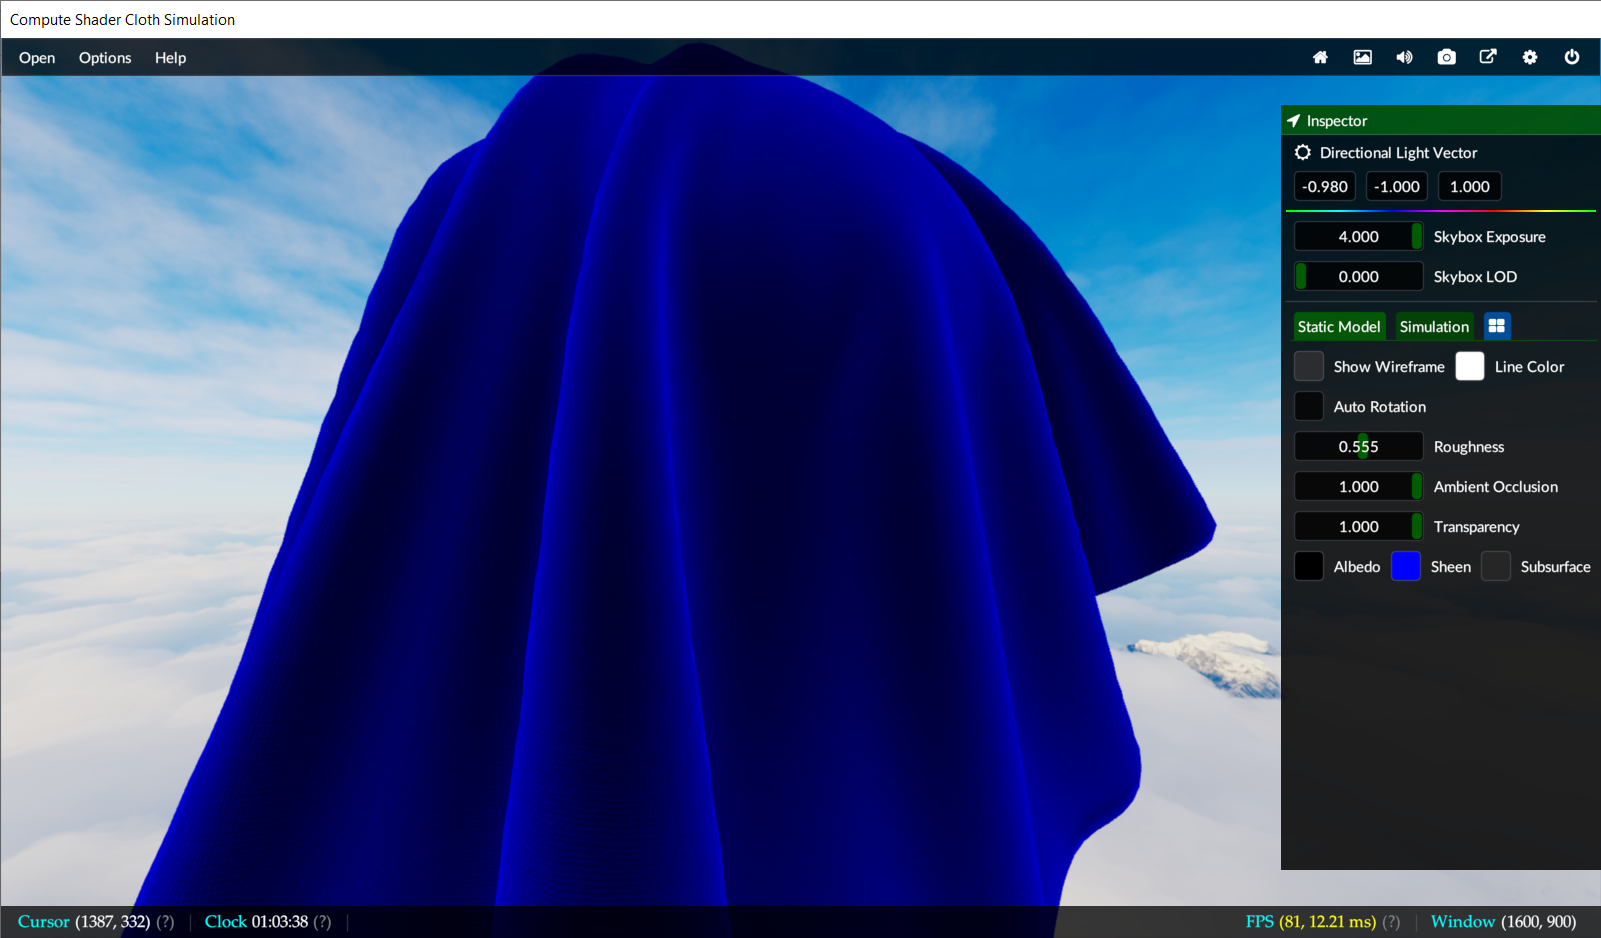
\includegraphics[width=0.8\linewidth]{66.png}
%\end{figure}
%\solution\\
%Figure 2(a) is a unit square bitmap, where $0 \leq s,t \leq 1$.\\
%Figure 2(b) is a curved part of the cylinder, suppose the height is $h$, any point on the surface can be represented by:
%\begin{align*}
%x &= rcos\theta \;\;(0 \leq \theta \leq \frac{\pi}{2})\\
%y &= rsin\theta \;\;(0 \leq \theta \leq \frac{\pi}{2})\\
%z &= kh \;\;(0 \leq k \leq 1)
%\end{align*}
%
%As $s$ goes from 0 to 1, we want $\theta$ to go from 0 to $\frac{\pi}{2}$.\\
%As $t$ goes from 0 to 1, we want $k$ to go from 0 to 1, so that $z$ goes from 0 to $h$.
%
%Hence, the texture image can be mapped to the cylinder patch via
%\begin{align*}
%s &= \theta / \frac{\pi}{2} = \frac{2\theta}{\pi}\\
%t &= k
%\end{align*}































%\end{enumerate}

\end{document}
